

\renewcommand{\appendixname}{Anexo}
\renewcommand{\appendixtocname}{Anexo}
\renewcommand{\appendixpagename}{Anexo}

\appendix

\chapter{Adquisición de datos}


\begin{figure}[H]
\centering
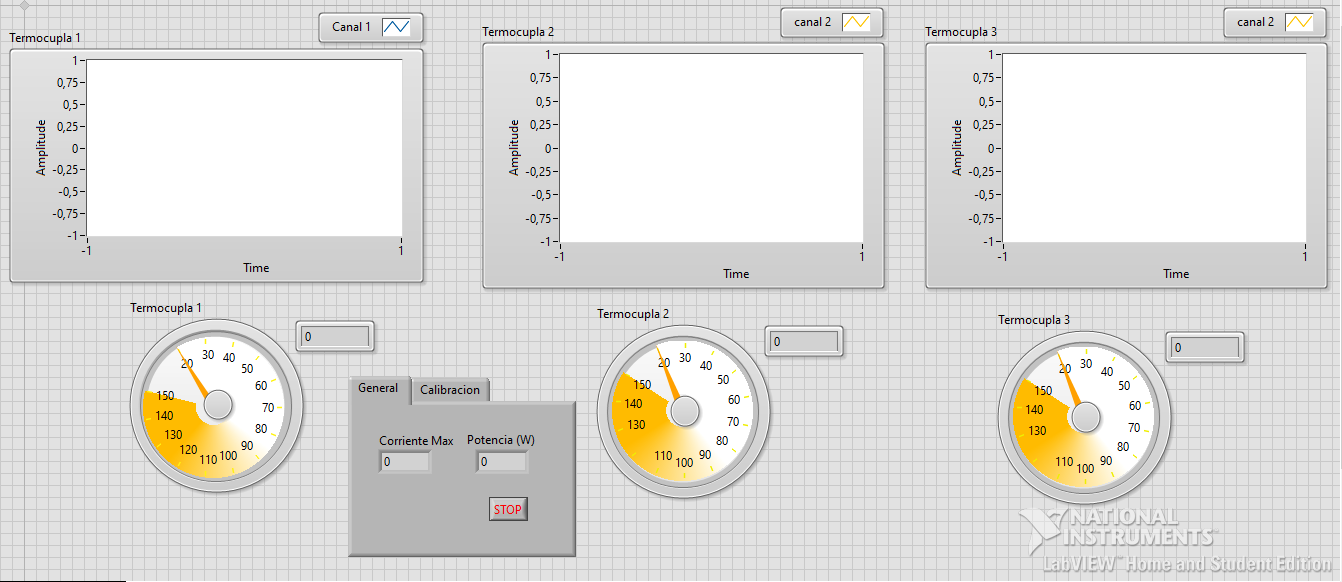
\includegraphics[width=\linewidth]{Figuras/lab3.png} % no debe ser mas grande que el texto
\caption{Panel Frontal de la Adquisición de Datos}
\centering
Fuente:Elaboración propia
\label{anexo2}
\end{figure}

\vfill

\begin{figure}[h]
\centering
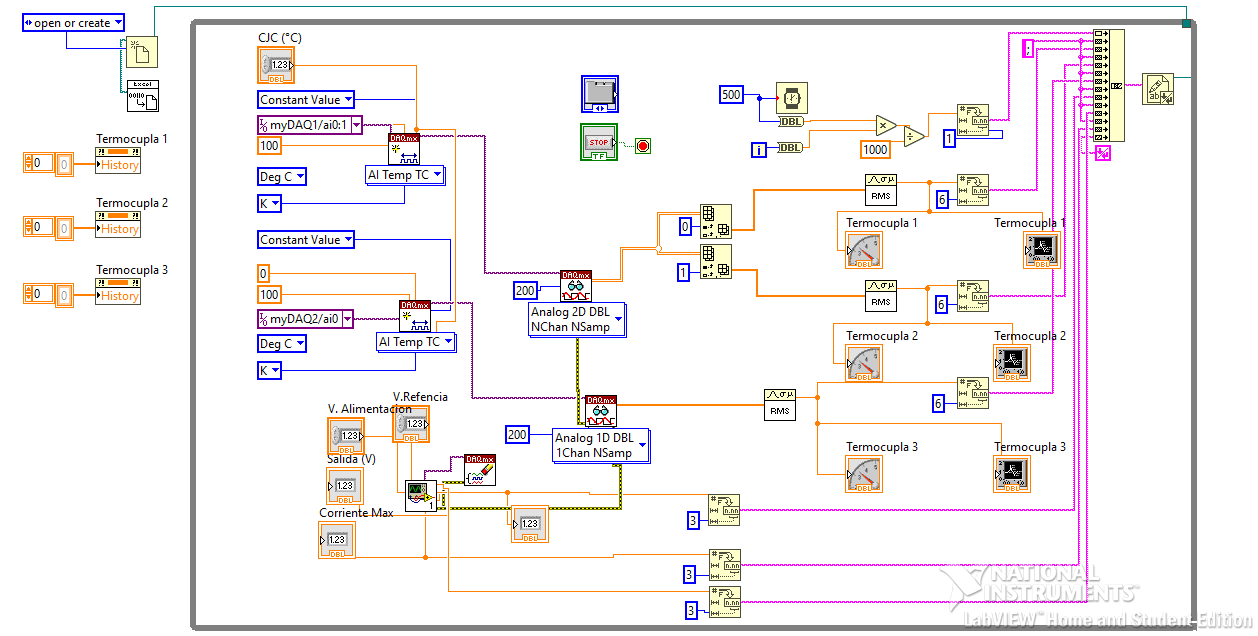
\includegraphics[width=\linewidth]{Figuras/lab1.png}
\caption{Algoritmo de adquisición de datos, Labview}
\centering
Fuente:Elaboración propia
\label{anexo3}
\end{figure}

\vfill
\begin{figure}[H]
\centering
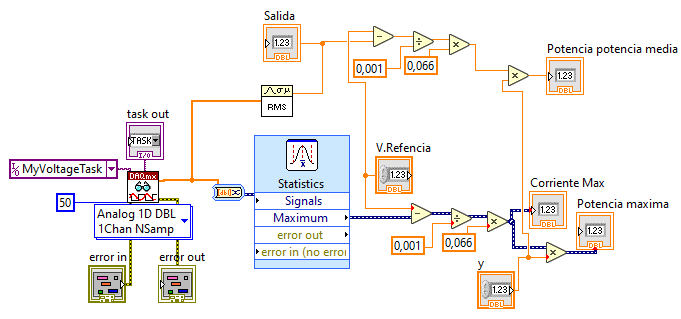
\includegraphics[width=\linewidth]{Figuras/lab2.png} % se salia de la página
\caption{Algoritmo de medición de corriente}
\centering
Fuente:Elaboración propia
\label{anexo4}
\end{figure}
\vfill

\vfill

\begin{figure}[H]
\centering
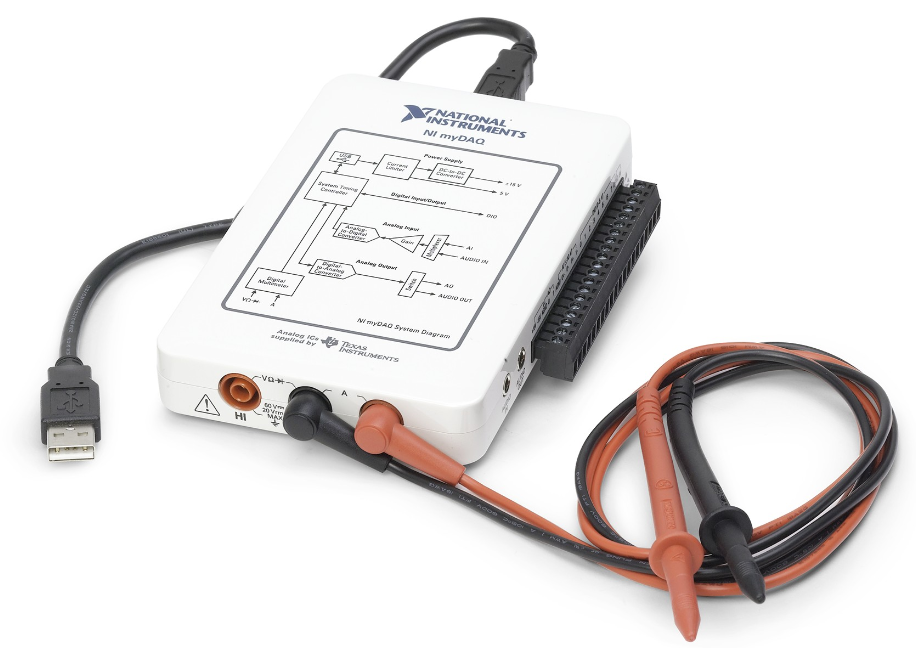
\includegraphics[scale=0.5]{Figuras/daq.png}
\caption{Algoritmo de medición de corriente}

Fuente:\cite{daq}
\label{anexo5}
\end{figure}

\begin{figure}[H]
\centering
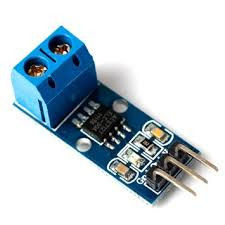
\includegraphics[scale=0.9]{Figuras/asc712.jpg}
\caption{Algoritmo de medición de corriente}
Fuente:\cite{asc712}
\label{anexo6}
\end{figure}

\chapter{Algoritmos de Simulación}


\begin{figure}[H]
\centering
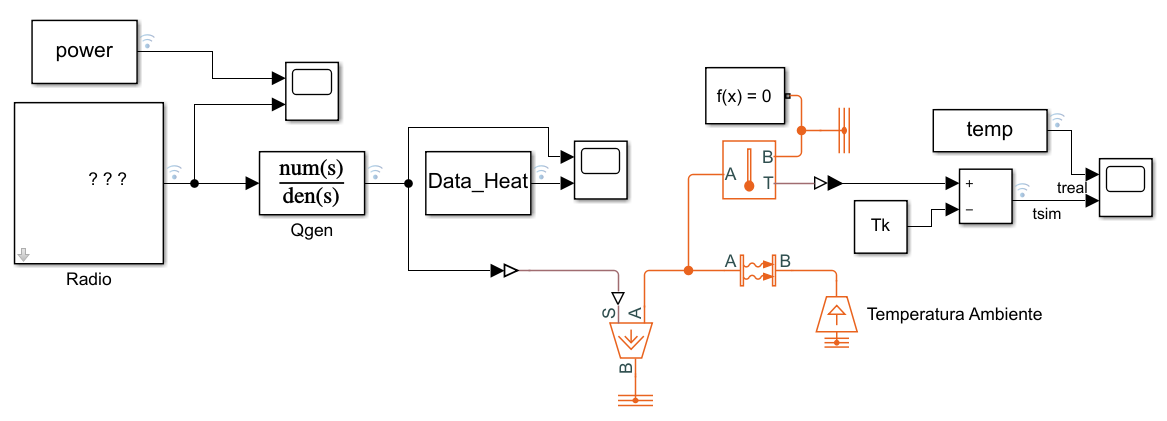
\includegraphics[scale=0.5]{Figuras/modelo_radio.png}
\caption{Algoritmo del modelo para el radio}
\centering
Fuente: Elaboración Propia
\label{anexo7}
\end{figure}

\begin{figure}[H]
\centering
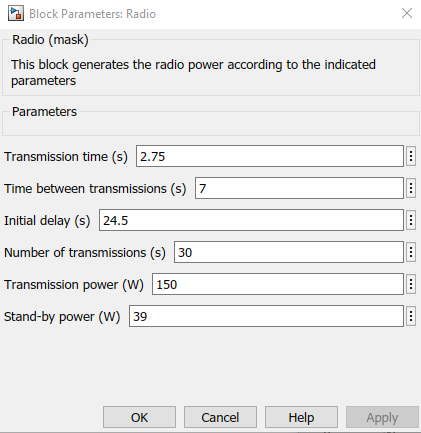
\includegraphics[scale=0.7]{Figuras/parametros_resultado.png}
\caption{Parámetros de entrada del modelo}
Fuente: Elaboración Propia
\label{anexo8}
\end{figure}


\begin{figure}[H]
\centering
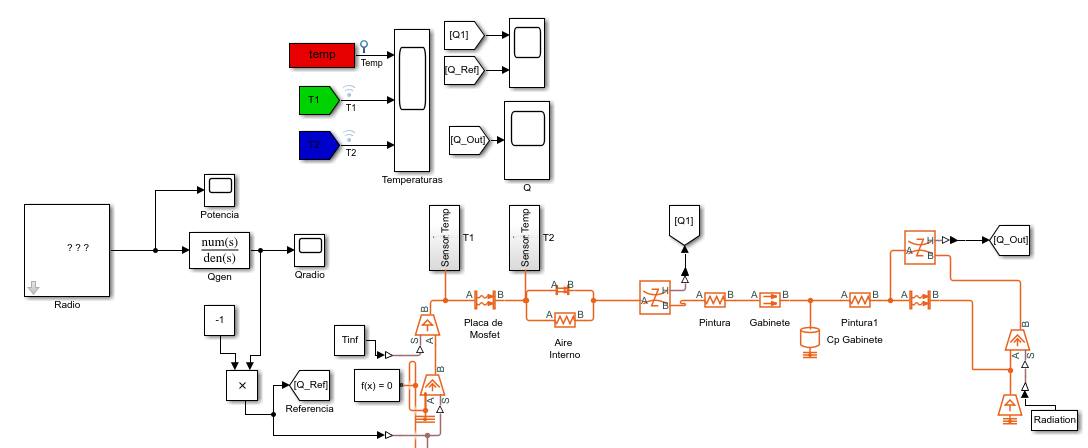
\includegraphics[width=\linewidth]{Figuras/Algoritmo_GTR.png} %nunca debe ser mas grande que los margenes, aqui mejor usar \linewidth
\caption{Algoritmo para la GRT}
Fuente: Elaboración Propia
\label{anexo10}
\end{figure}

\begin{figure}[H]
\centering
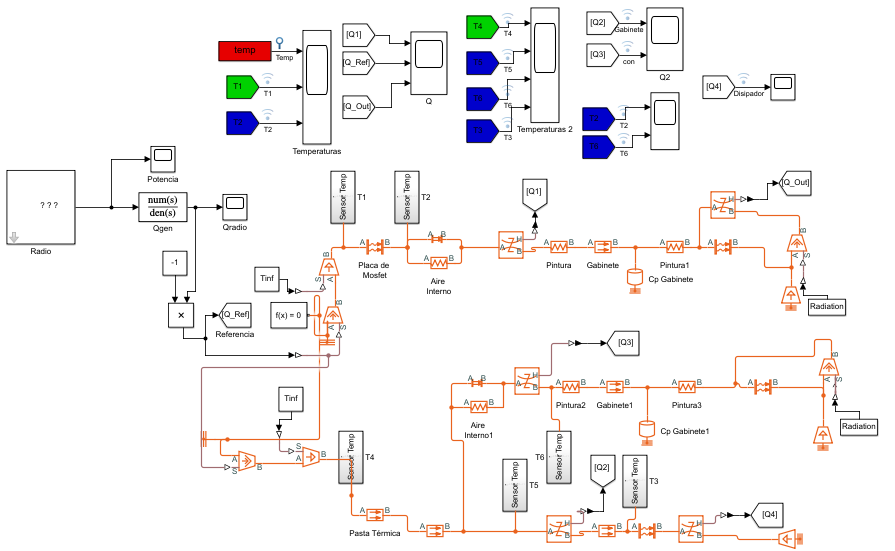
\includegraphics[scale=0.6]{Figuras/algoritmo_final.png}
\caption{Algoritmo con disipador de calor}
Fuente: Elaboración Propia
\label{anexo11}
\end{figure}

\chapter{Montaje del experimento}

\begin{figure}[H]
\centering
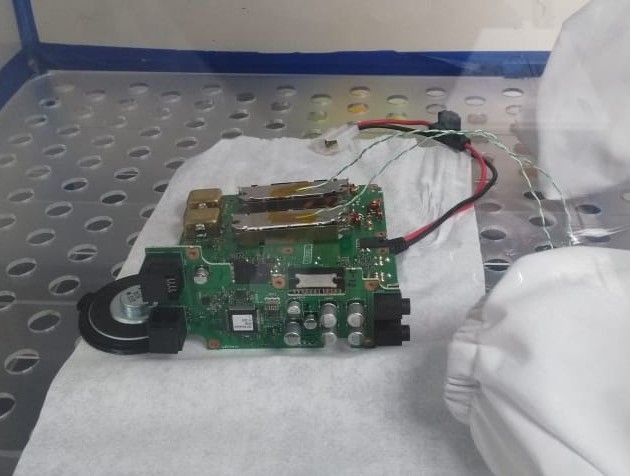
\includegraphics[scale=0.6]{Figuras/Montaje_2.jpeg}
\caption{Posición de las Termocuplas, vista lateral}
Fuente: Elaboración Propia
\label{anexo12}
\end{figure}

\begin{figure}[H]
\centering
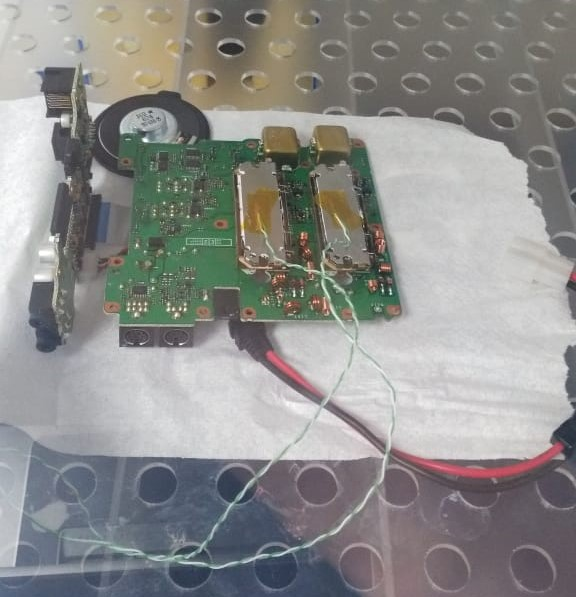
\includegraphics[scale=0.5]{Figuras/Montaje_3.jpeg}
\caption{Posición de las Termocuplas, vista frontal}
Fuente: Elaboración Propia
\label{anexo13}
\end{figure}

\begin{figure}[H]
\centering
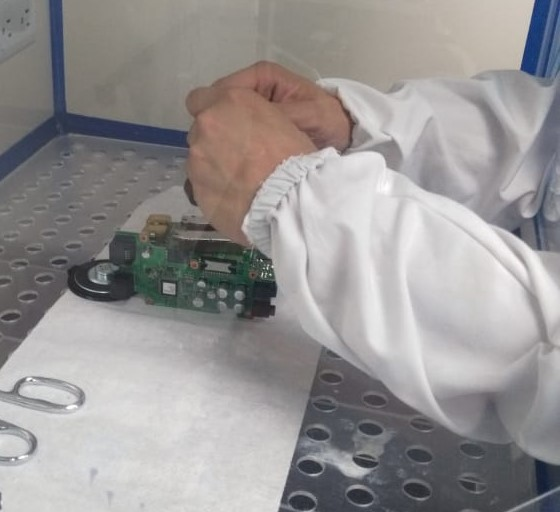
\includegraphics[scale=0.5]{Figuras/Montaje_4.jpeg}
\caption{Proceso de montaje para las termocuplas}
Fuente: Elaboración Propia
\label{anexo14}
\end{figure}

\begin{figure}[H]
\centering
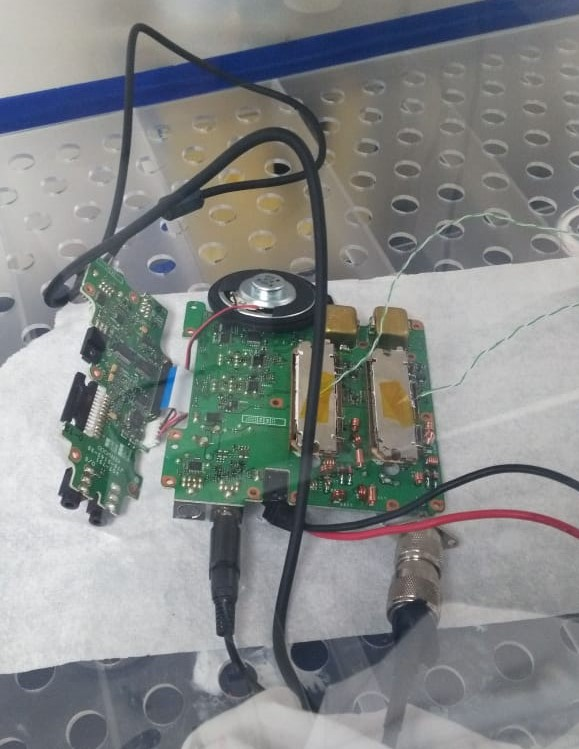
\includegraphics[scale=0.5]{Figuras/Montaje_6.jpeg}
\caption{Conexión de puertos}
Fuente: Elaboración Propia
\label{anexo15}
\end{figure}

\chapter{Radio Transmisor}

\begin{figure}[H]
\centering
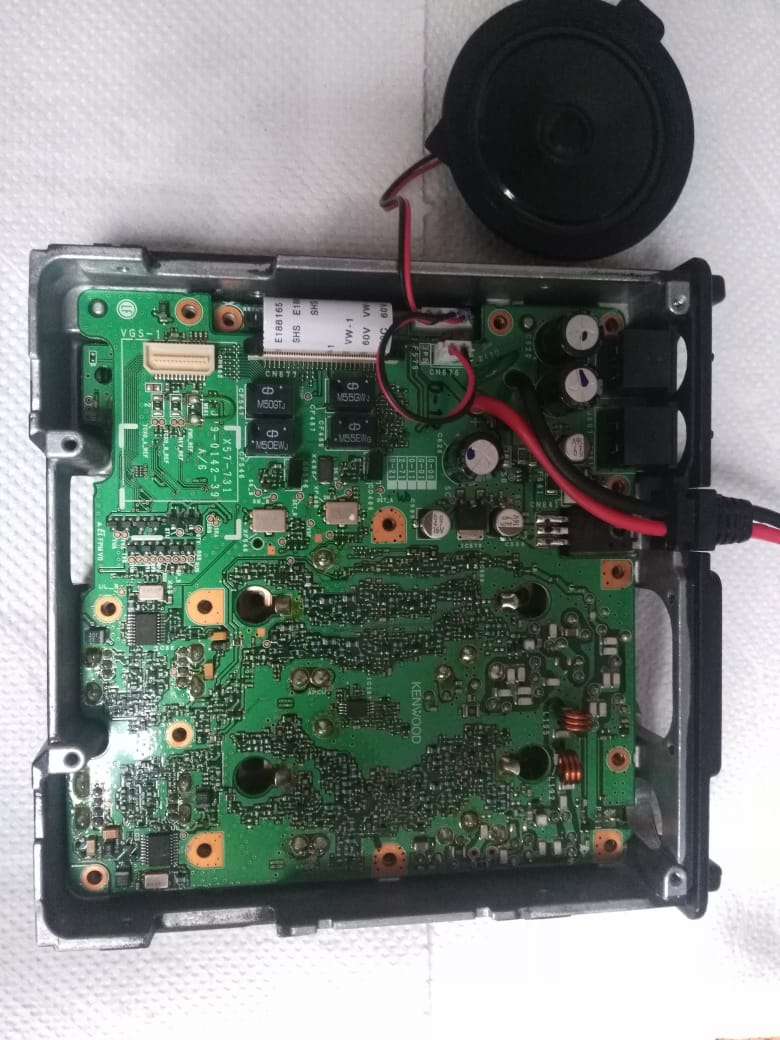
\includegraphics[scale=0.3]{Figuras/Radio_1.jpeg}
\caption{Radio en su carcasa}
Fuente: Elaboración Propia
\label{anexo16}
\end{figure}

\begin{figure}[H]
\centering
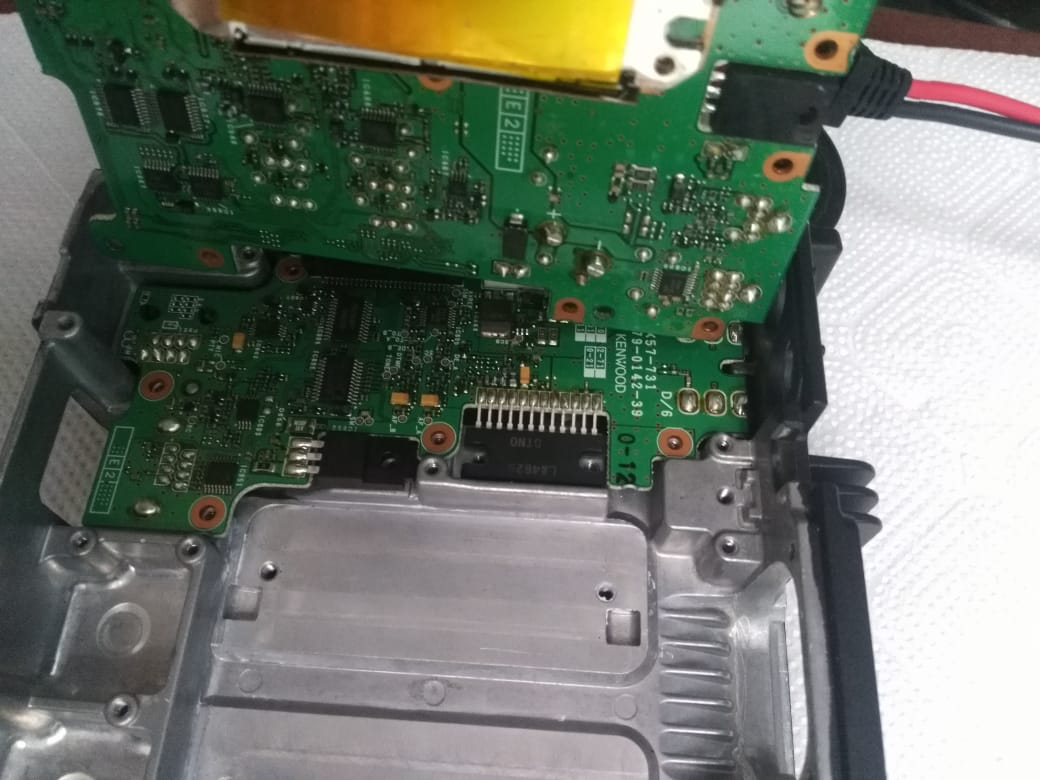
\includegraphics[scale=0.3]{Figuras/Radio_2.jpeg}
\caption{Disipador original y placa secundario}
Fuente: Elaboración Propia
\label{anexo17}
\end{figure}

\begin{figure}[H]
\centering
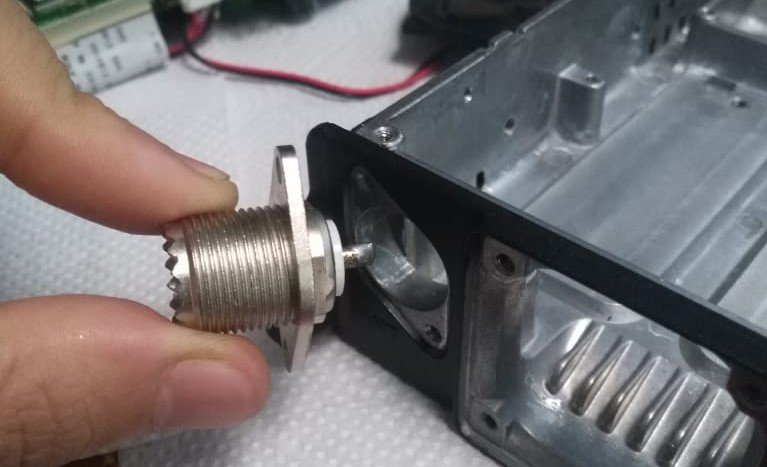
\includegraphics[scale=0.6]{Figuras/Radio_3.jpeg}
\caption{Disposición del conector de la antena }
Fuente: Elaboración Propia
\label{anexo18}
\end{figure}

\begin{figure}[H]
\centering
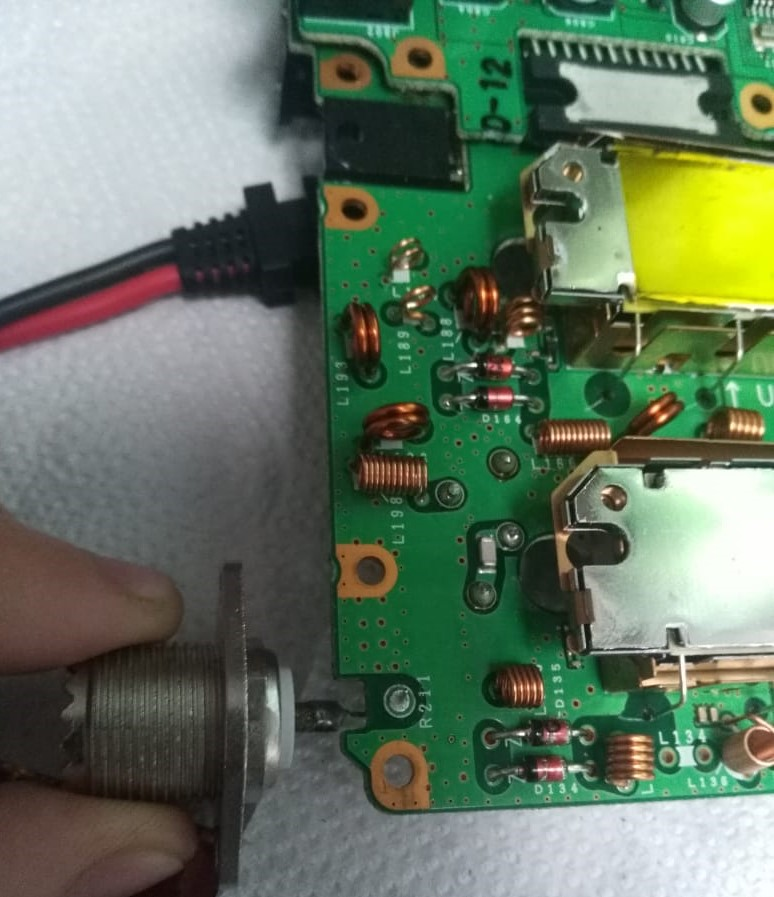
\includegraphics[scale=0.6]{Figuras/Radio_4.jpeg}
\caption{Conexión del conector de la antena al radio}
Fuente: Elaboración Propia
\label{anexo19}
\end{figure}

\chapter{Planos Constructivos}

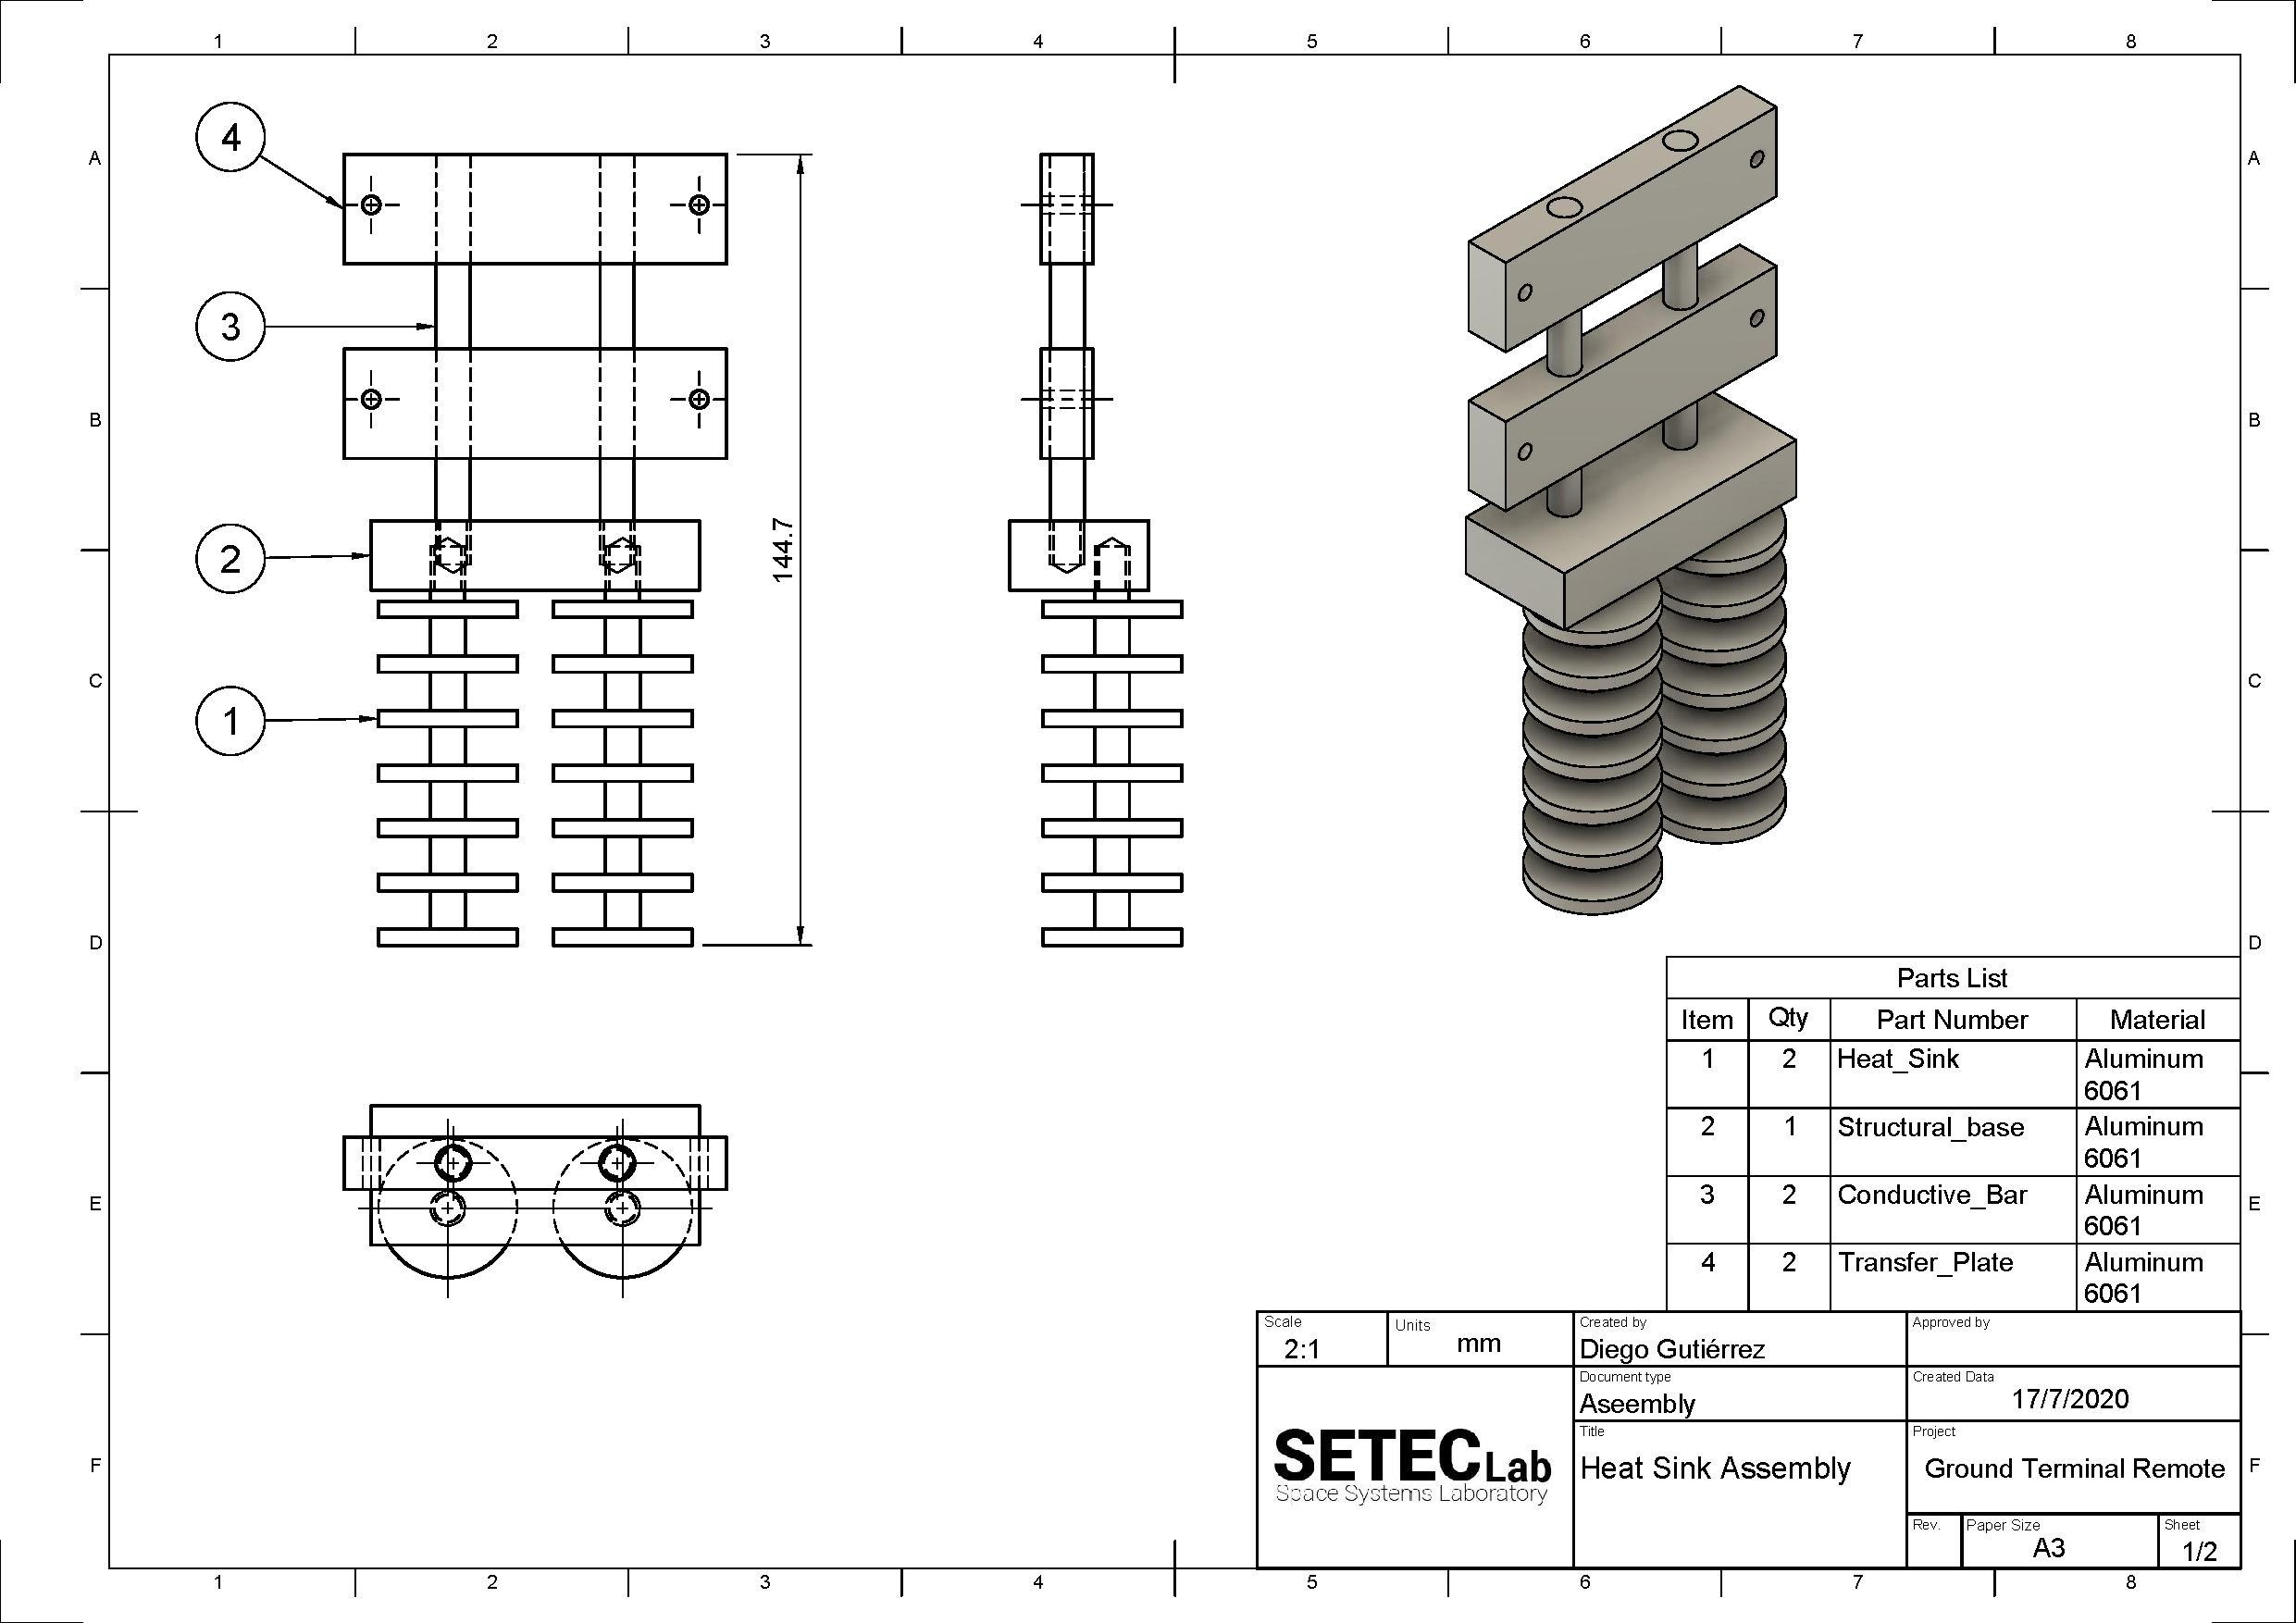
\includepdf[pages=-]{Heat_Sink_Planes}